\section{\textcolor{blue}{Hiện thực - Sprint1}} 
\subsection{Cài đặt repository (github, bitbucket, etc) cho việc quản lý phiên bản.}
Github repository của nhóm có thể được truy cập tại \href{https://github.com/ThangPham2508/SSPS\_HCMUT}{đây.}
\begin{figure}[H]
    \begin{center}
        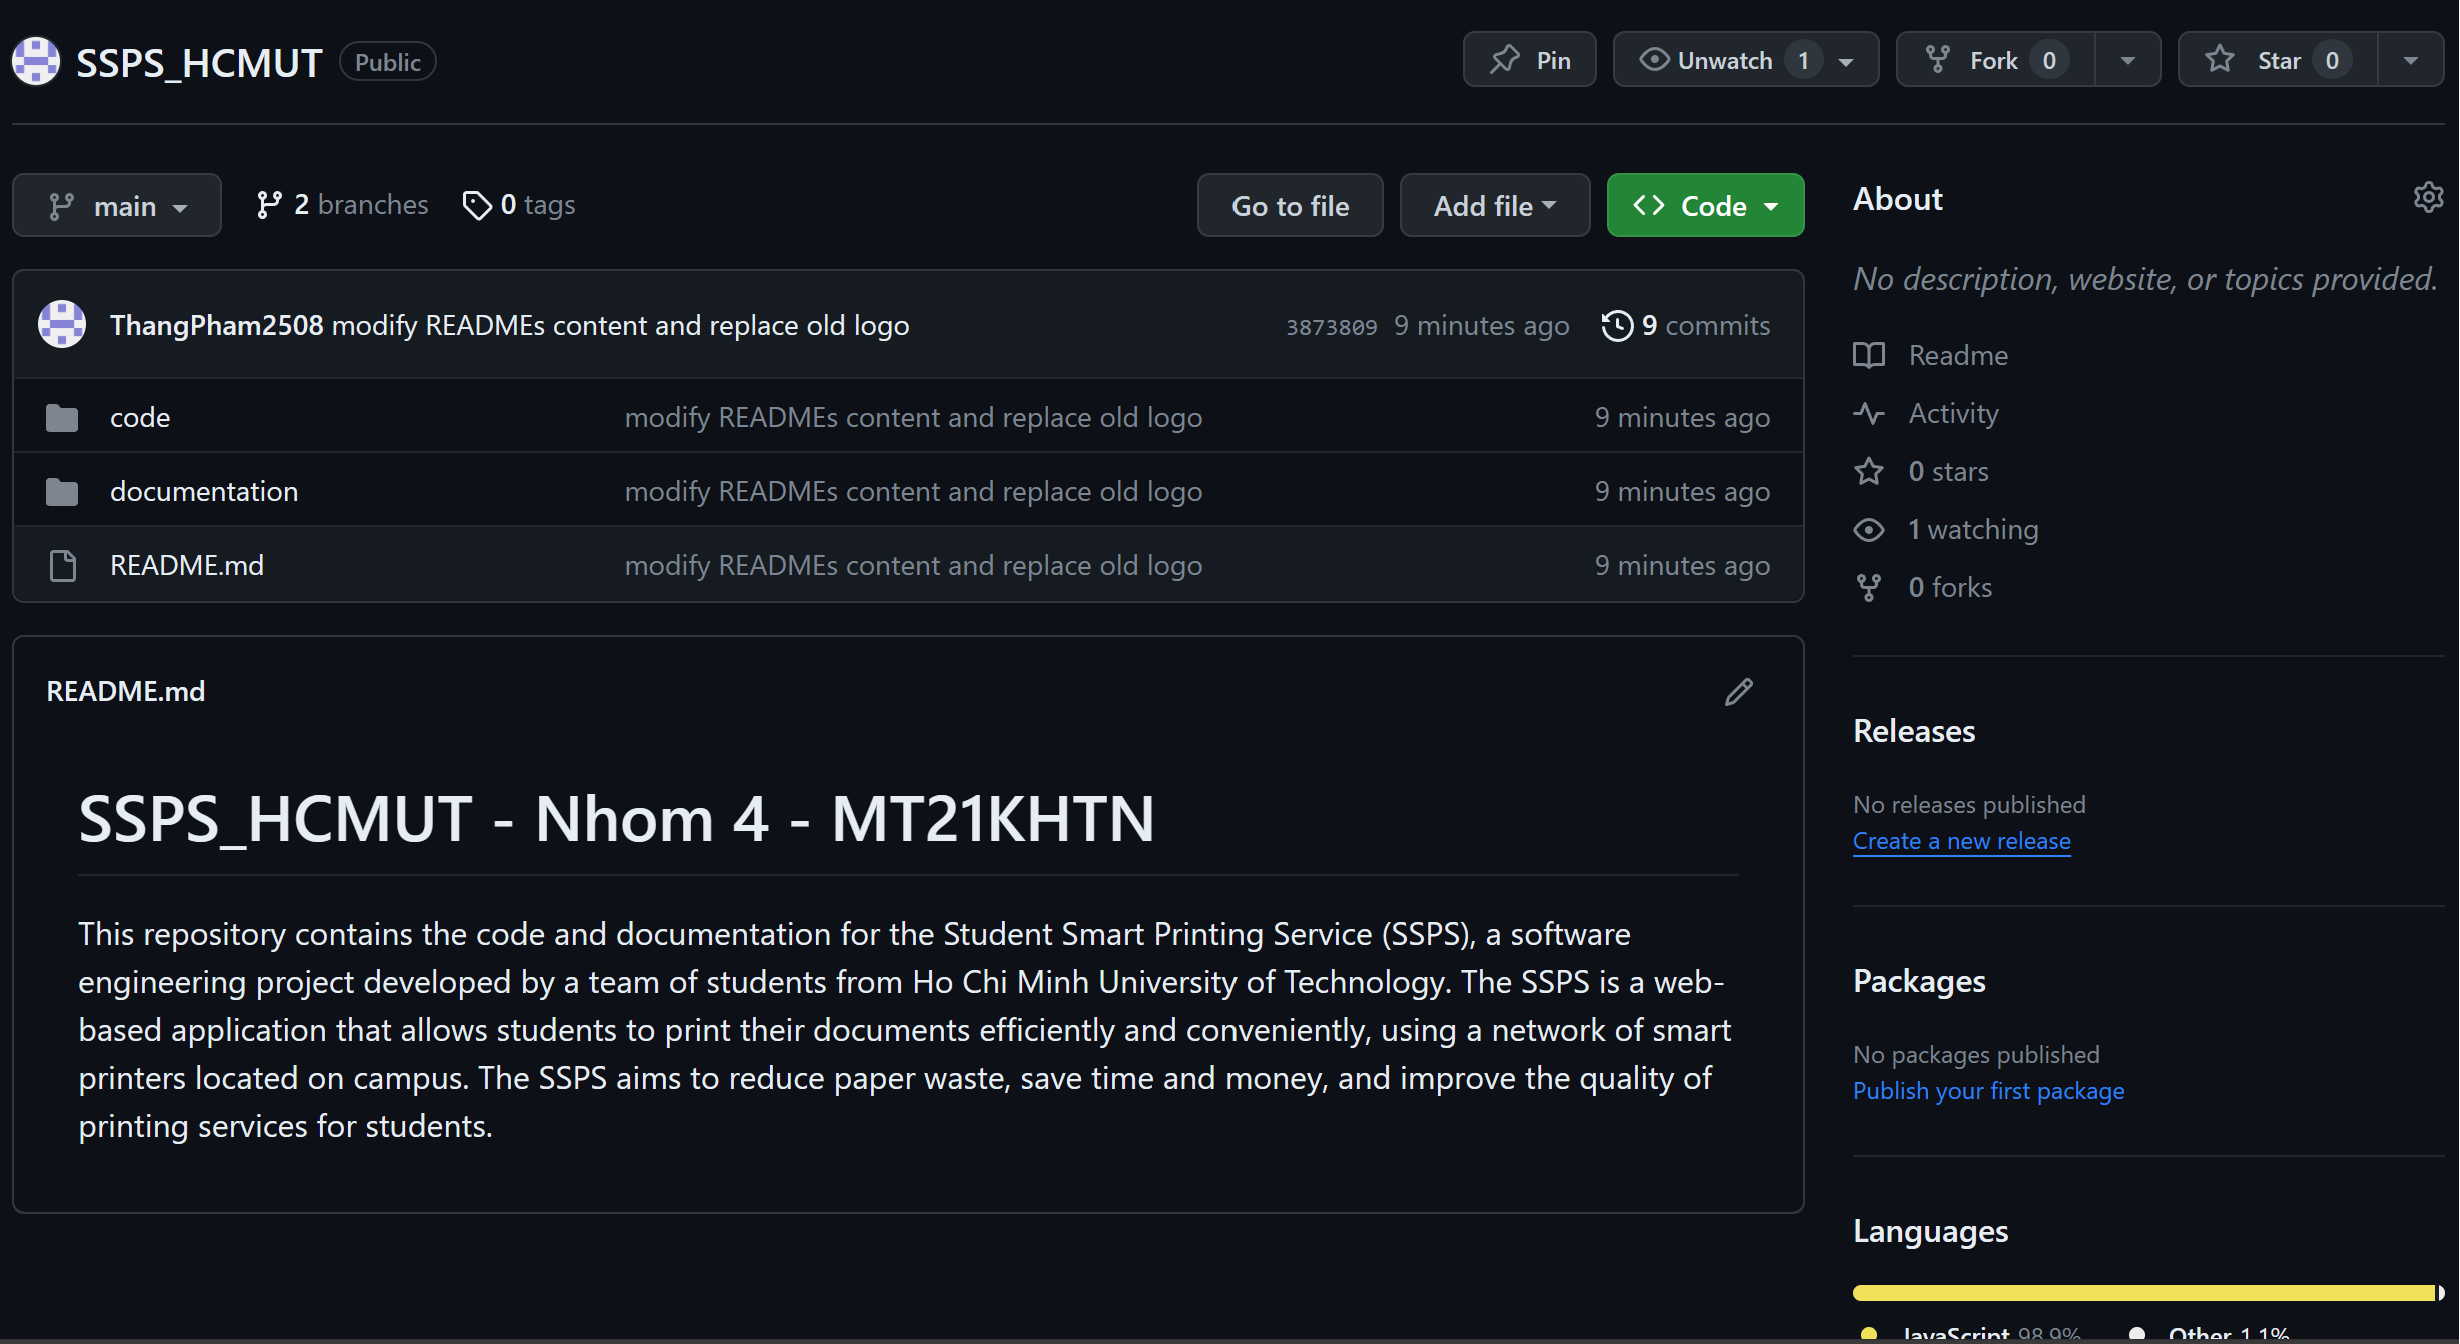
\includegraphics[width=1\textwidth]{Images/Github/github-main.png}
        \caption{Trang chủ Github Repository}
    \end{center}
\end{figure}
\subsection{Tài liệu và thư mục cho Requirement, System modelling và Architectural design.}
$\indent$Repository của dự án bao gồm hai thư mục chính:
\begin{itemize}
    \item \textbf{documentation:} thư mục này chứa các tài liệu liên quan đến dự án, cấu trúc thư mục bao gồm:
    \begin{figure}[H]
        \begin{center}
            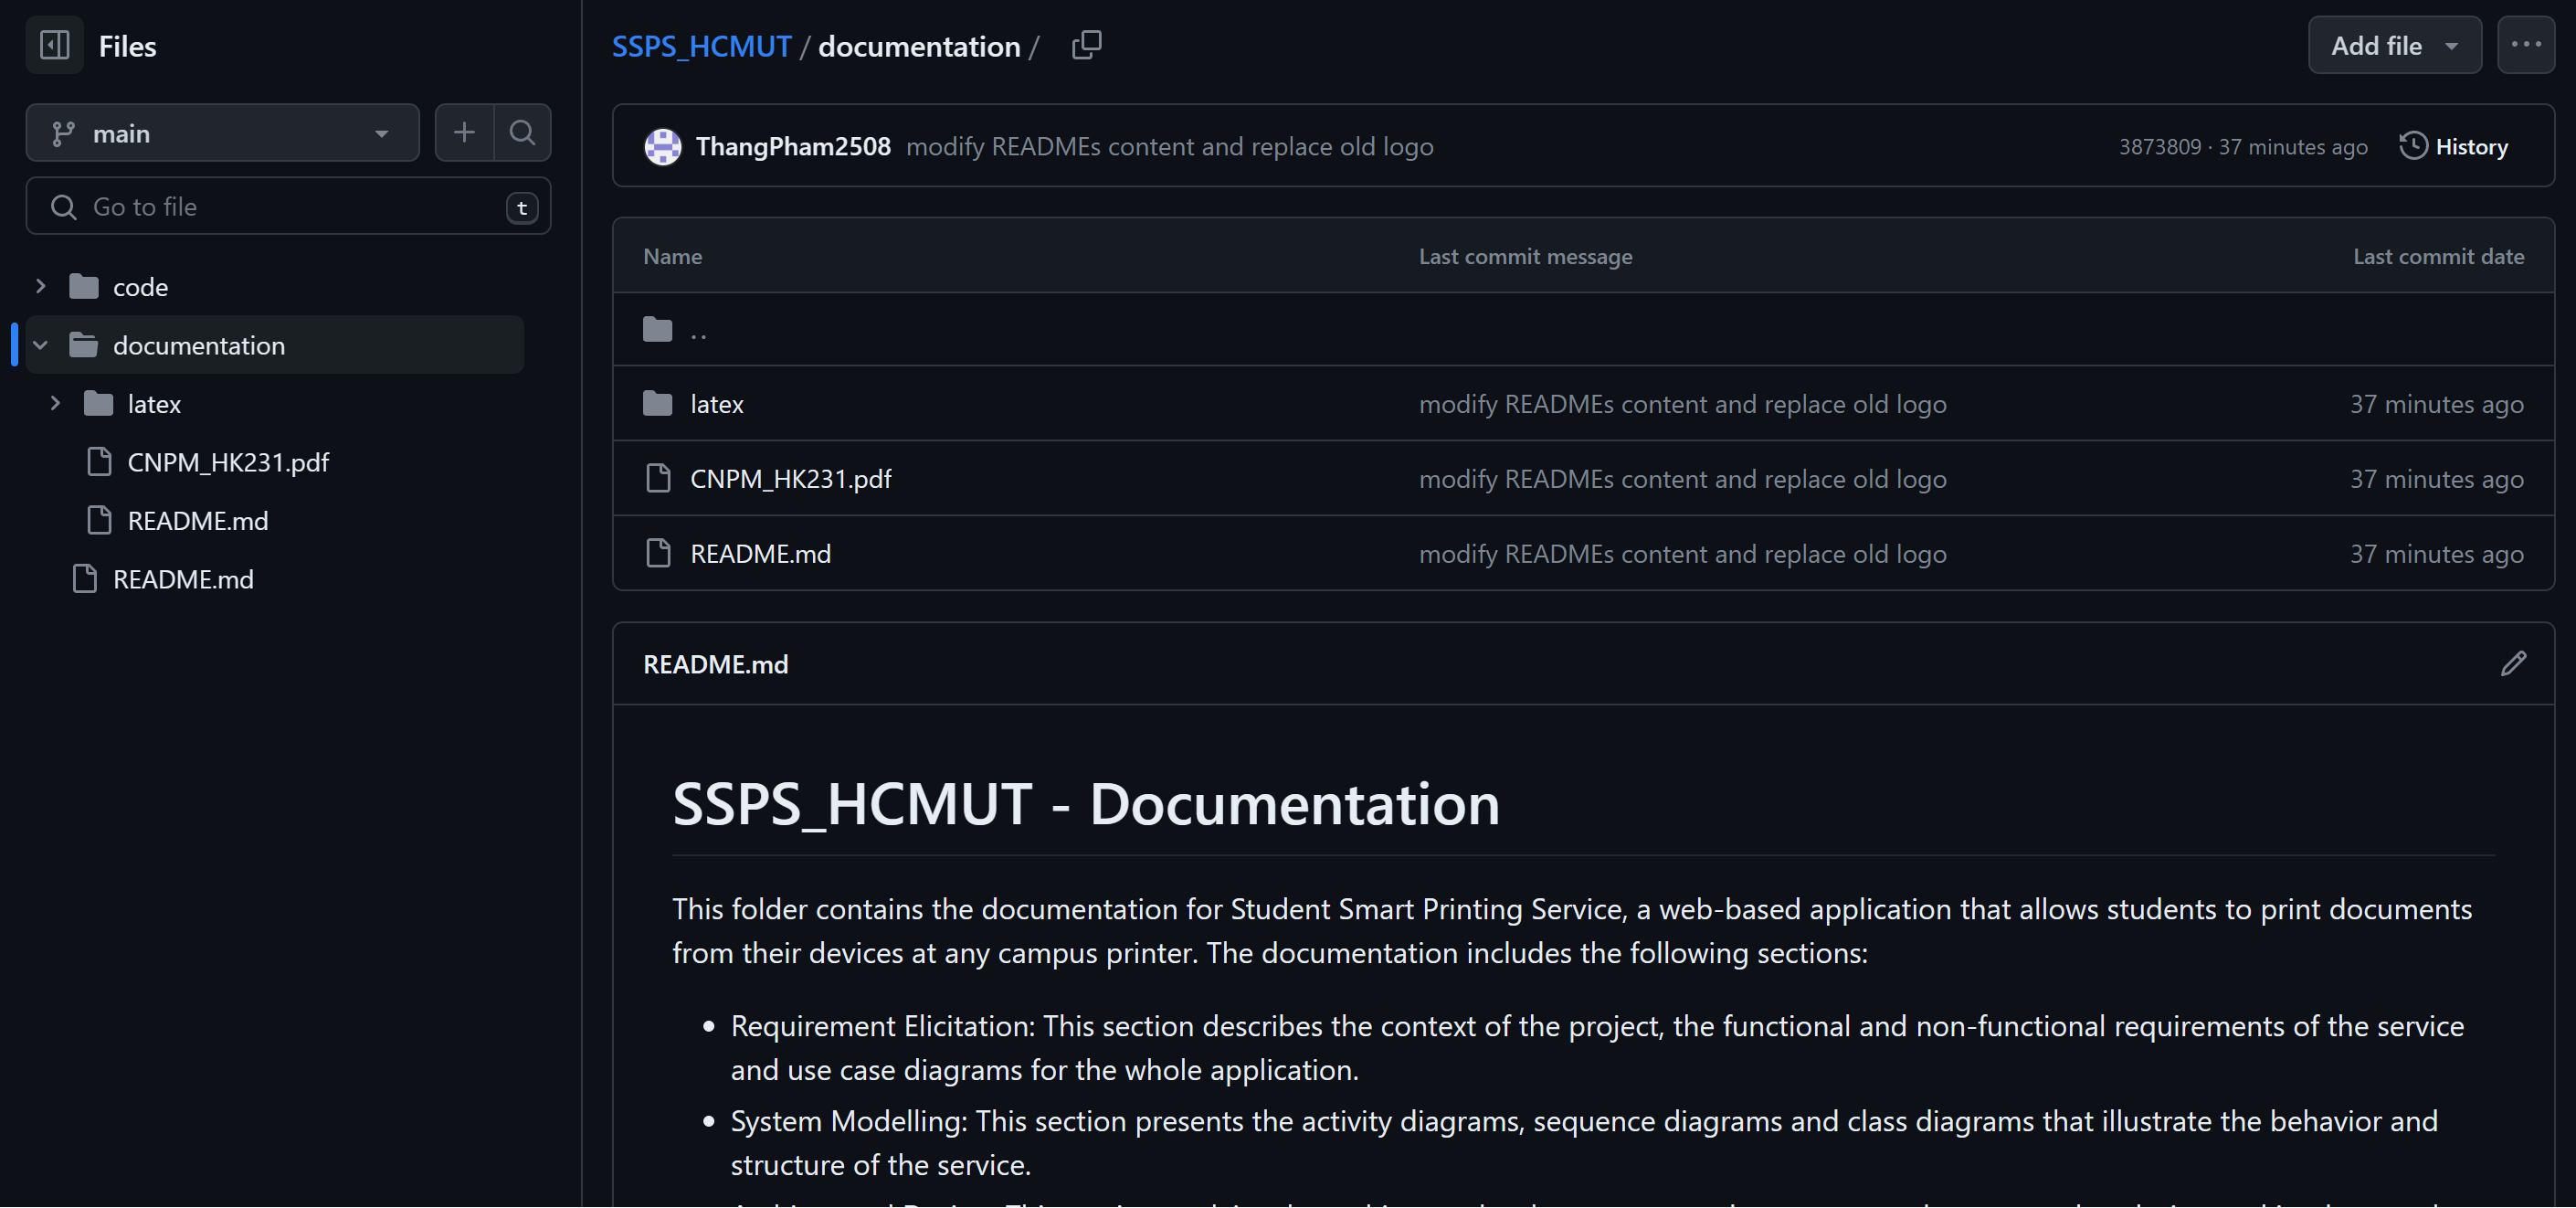
\includegraphics[width=1\textwidth]{Images/Github/github-documentation.png}
            \caption{Thư mục documentation}
        \end{center}
    \end{figure}
    \begin{itemize}
    \item Tệp pdf chính (CNPM\_HK231.pdf) chứa phiên bản hoàn chỉnh của tài liệu.
    \item \textbf{latex:} thư mục này chứa các tệp mã nguồn latex cho tài liệu, được tổ chức như sau:
    \begin{figure}[H]
        \begin{center}
            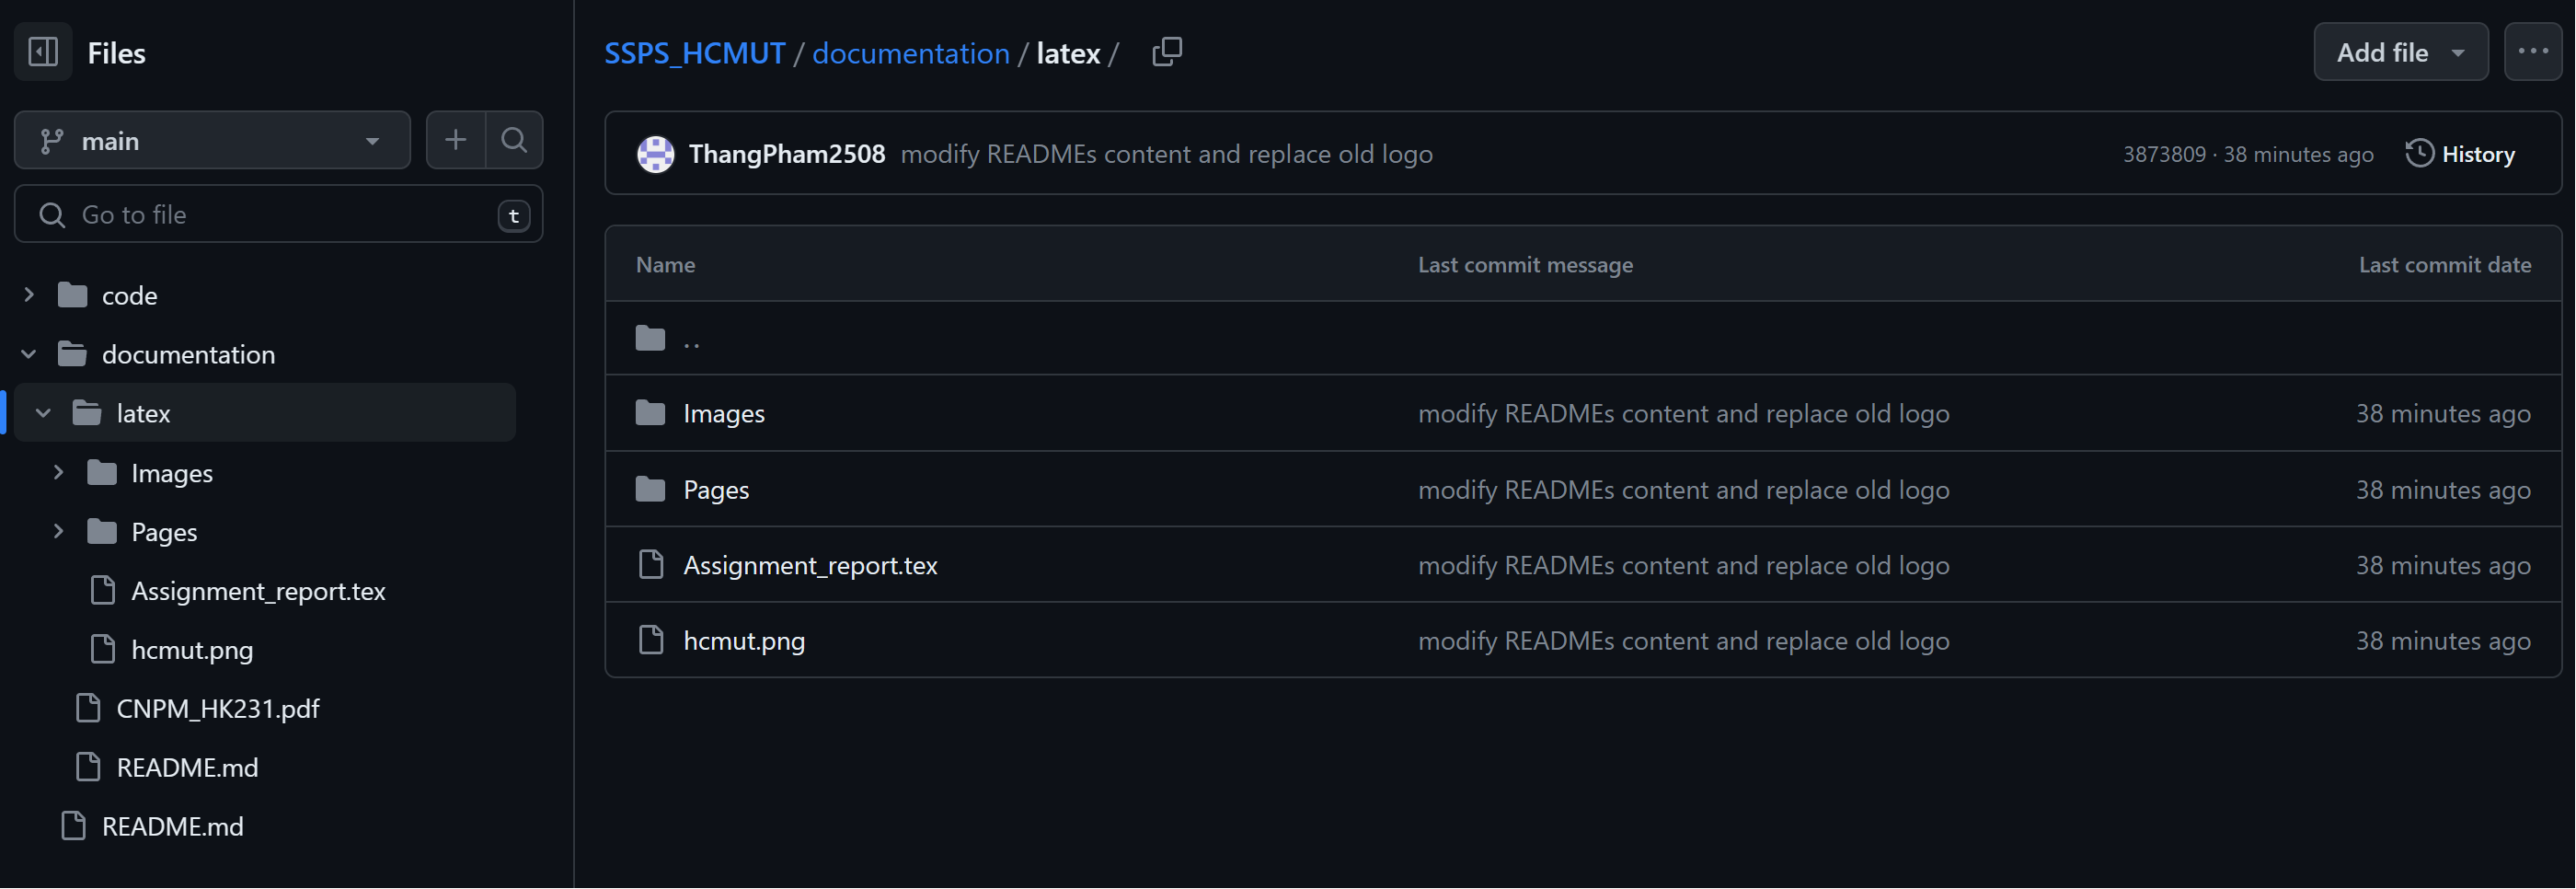
\includegraphics[width=1\textwidth]{Images/Github/github-latex.png}
            \caption{Thư mục latex}
        \end{center}
    \end{figure}
    \begin{itemize}
        \item \textbf{Images:} thư mục này chứa tất cả các hình ảnh được sử dụng trong tài liệu.
        \item \textbf{Pages:} thư mục này chứa các tệp latex riêng lẻ cho mỗi phần của tài liệu. Nó cũng chứa một tệp pdf của phần đó được trích xuất từ tệp pdf chính.
        \item Mỗi thư mục được mô tả ở trên được tổ chức theo các phần, bao gồm Requirement Elicitation, System Modelling và Architectural Design.
    \end{itemize}
    \begin{figure}[H]
        \begin{center}
            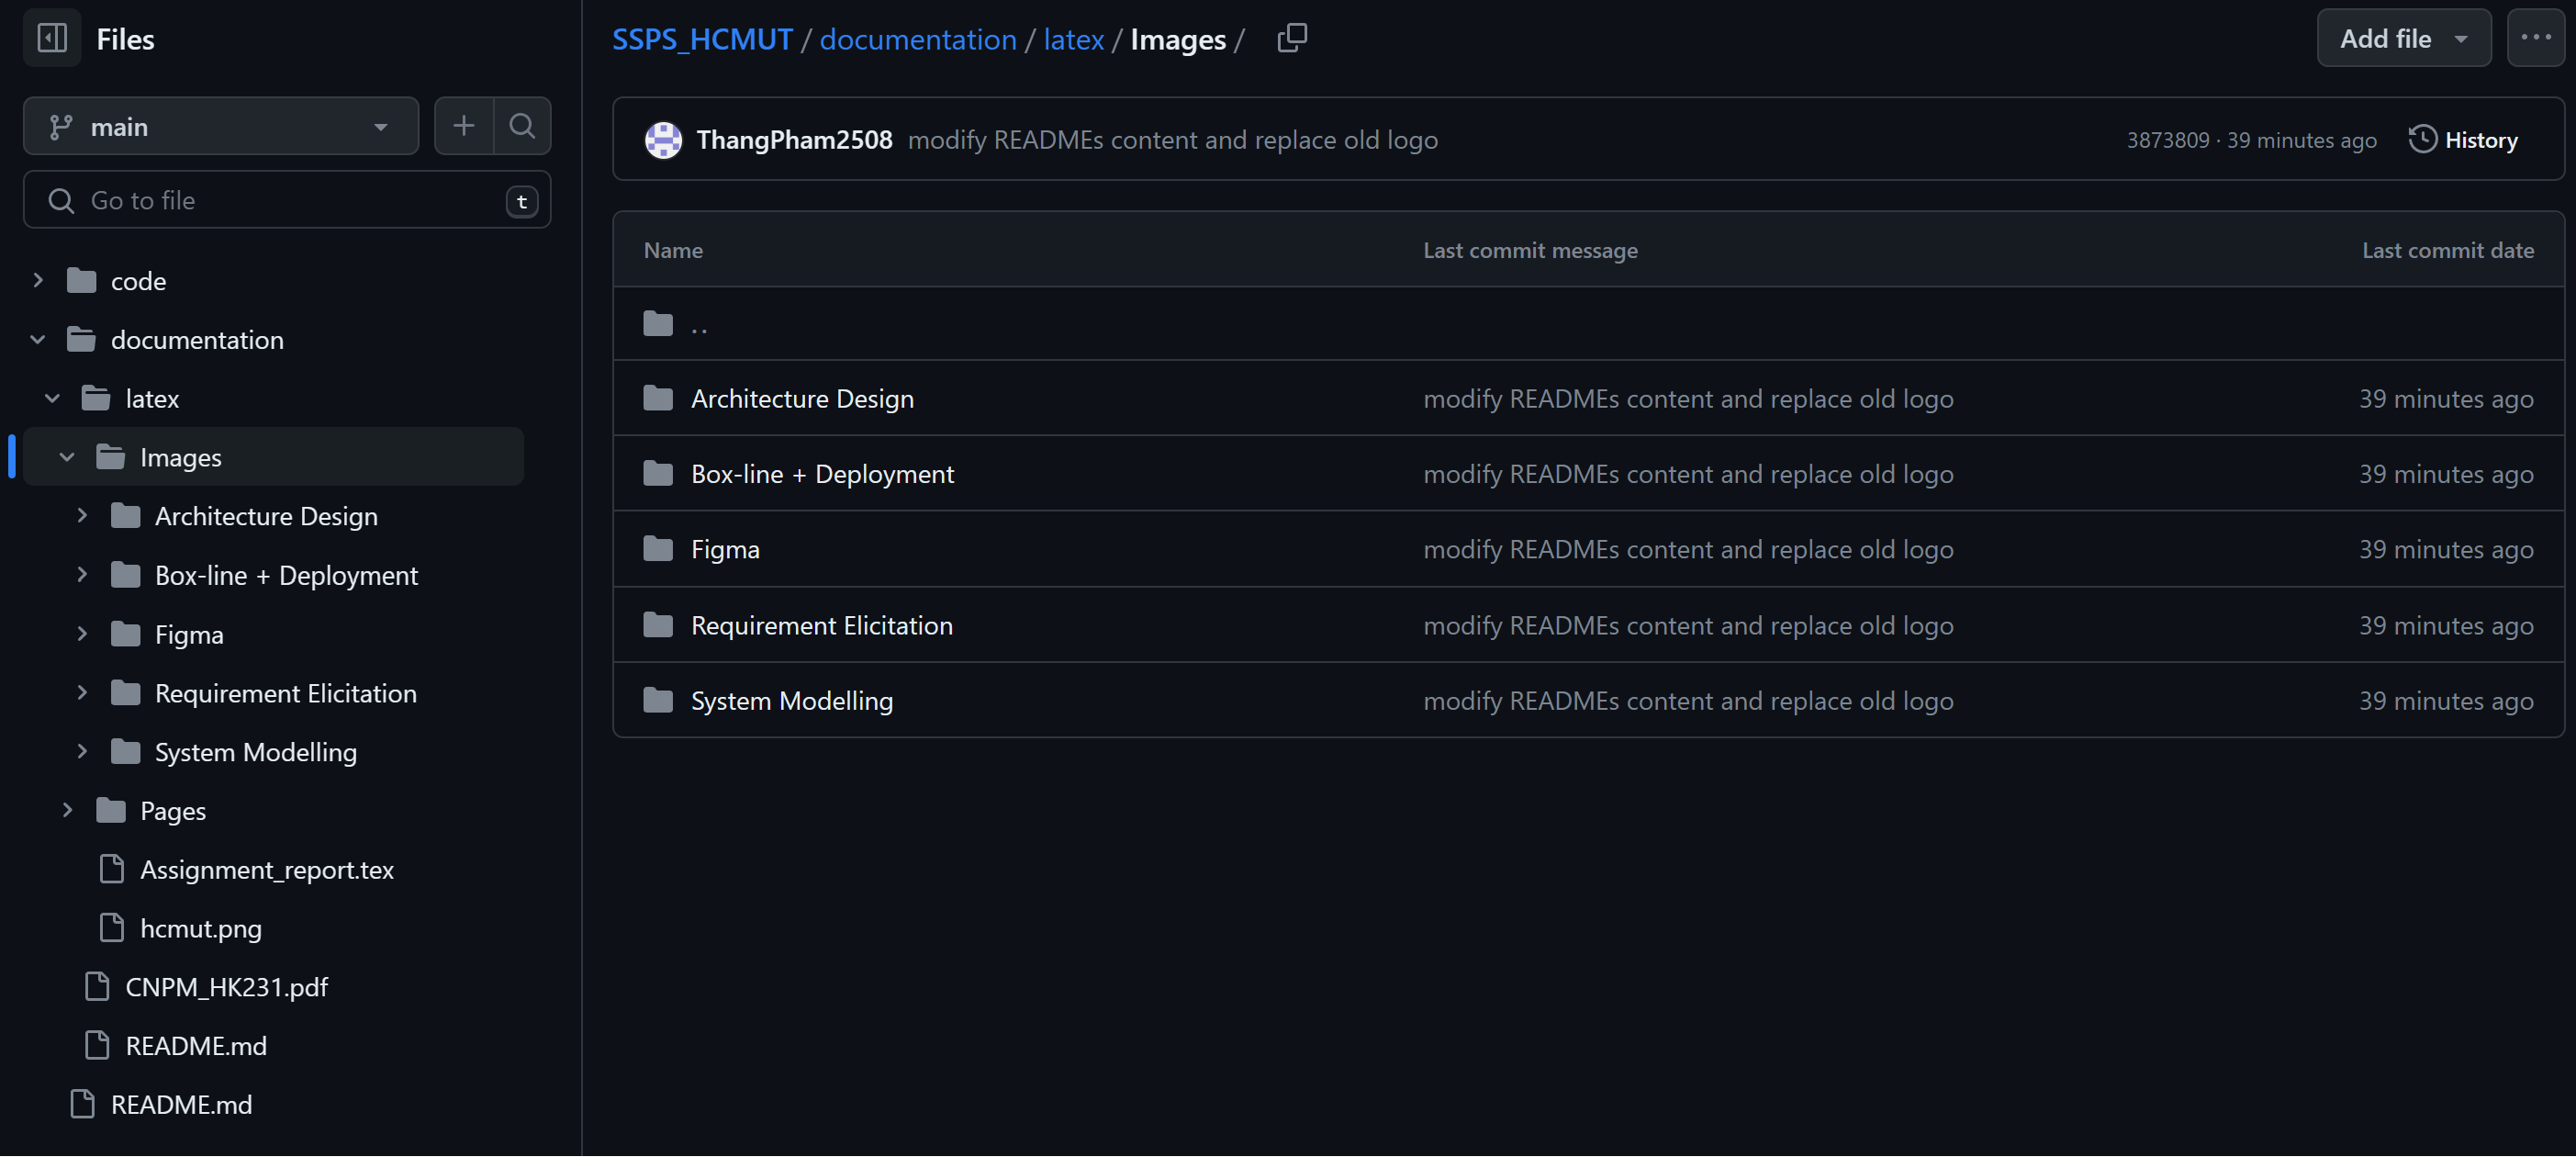
\includegraphics[width=1\textwidth]{Images/Github/github-images.png}
            \caption{Thư mục Images}
        \end{center}
    \end{figure}
    \begin{figure}[H]
        \begin{center}
            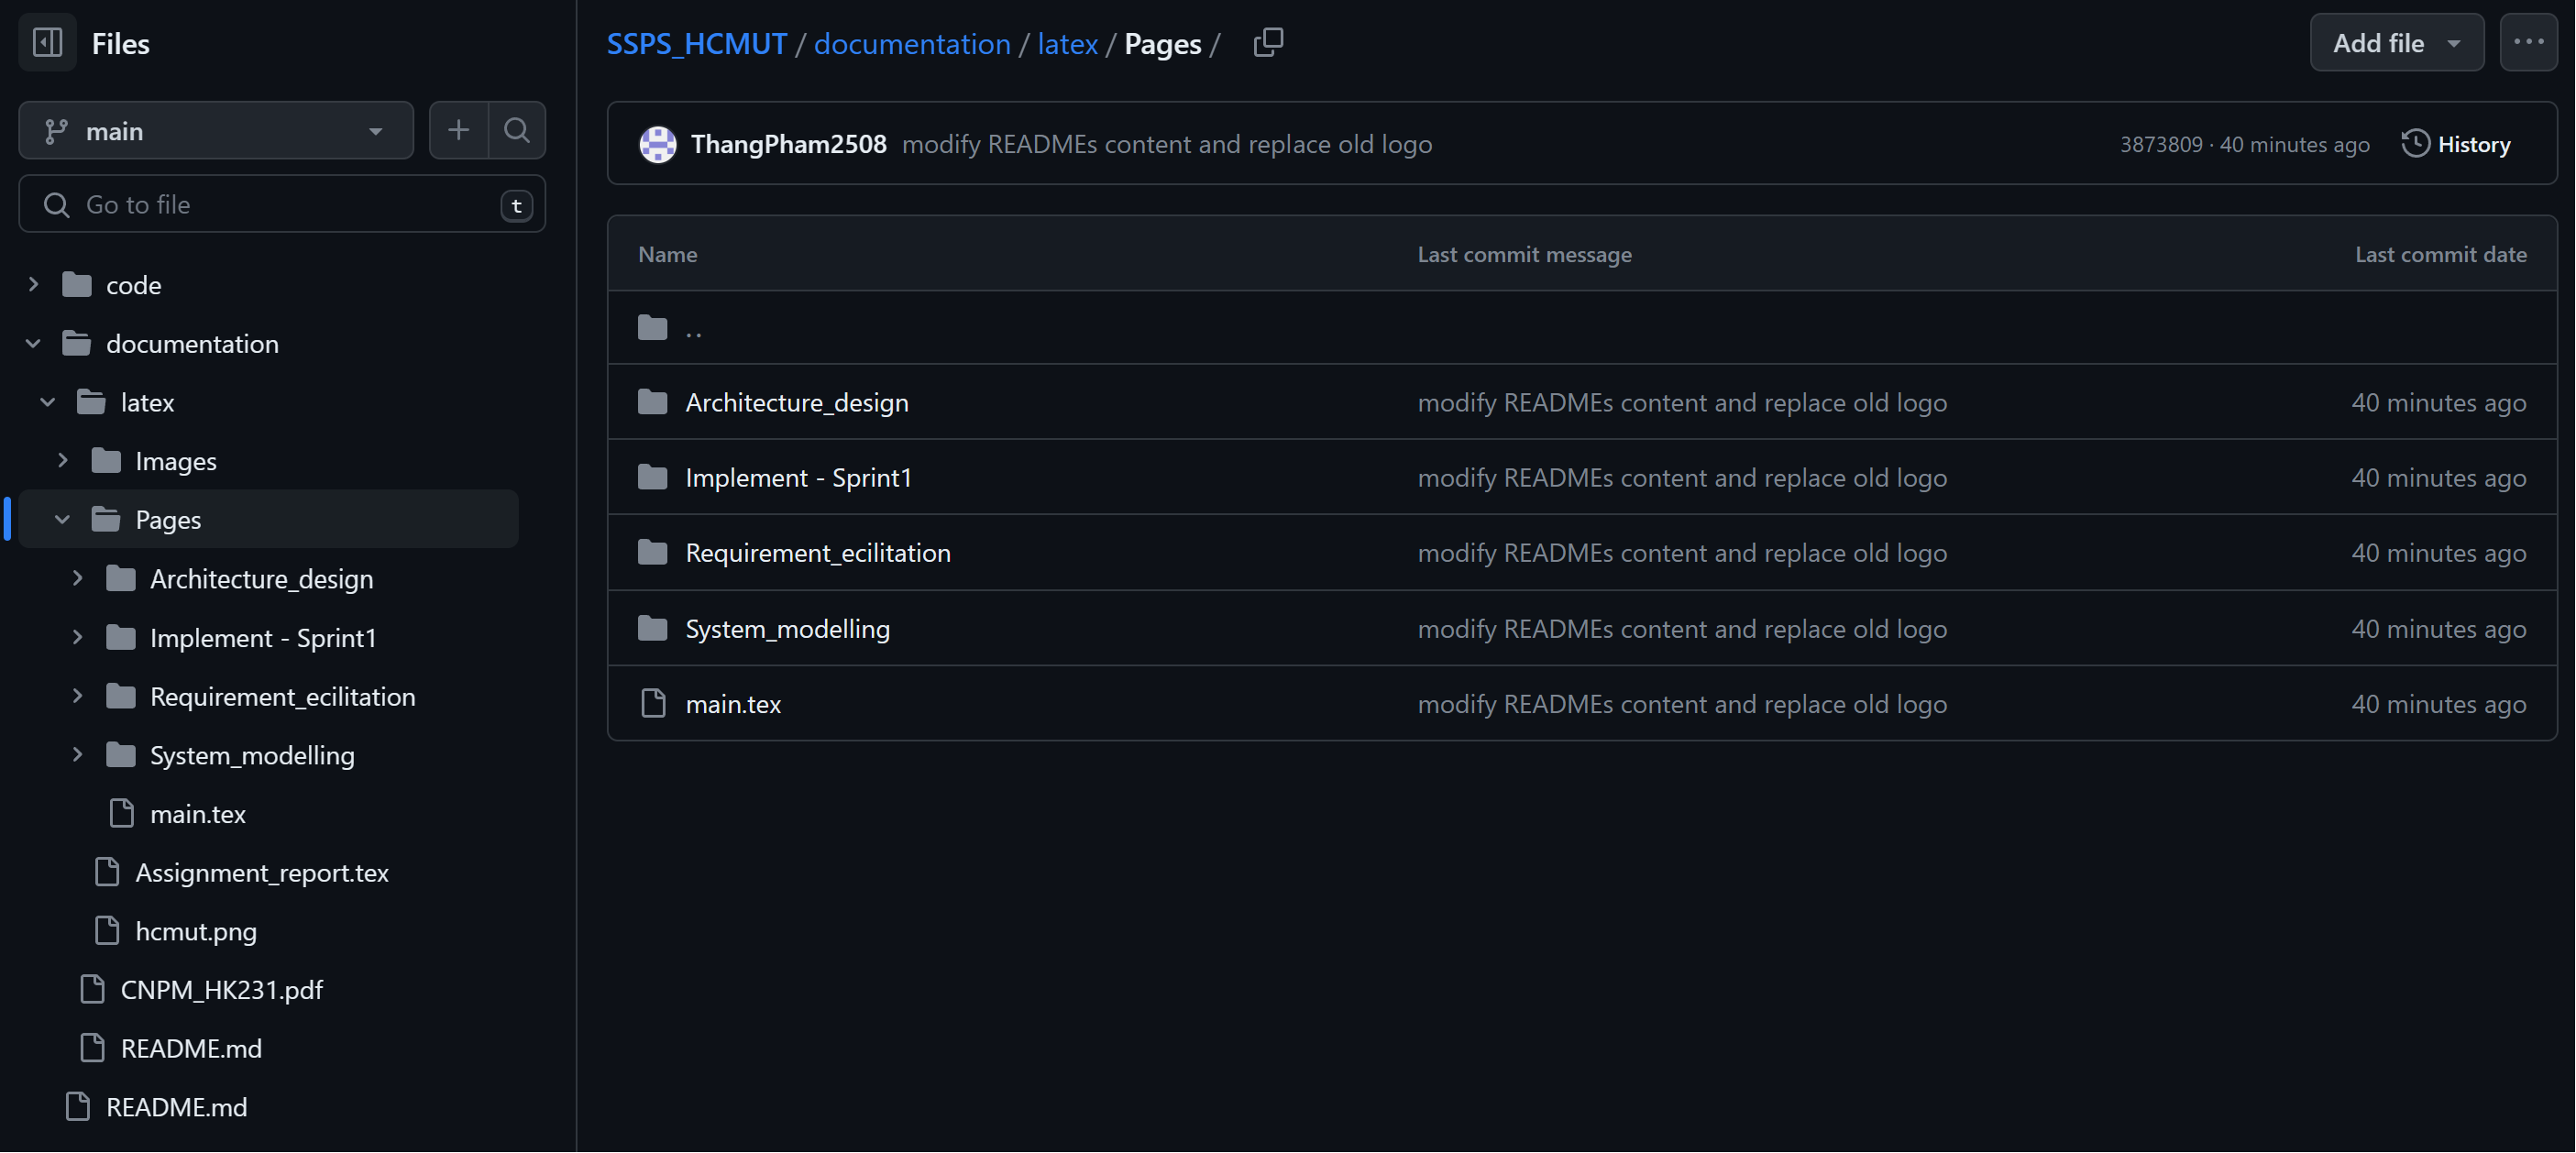
\includegraphics[width=1\textwidth]{Images/Github/github-pages.png}
            \caption{Thư mục Pages}
        \end{center}
    \end{figure}
\end{itemize}
\item \textbf{code:} thư mục này chứa mã nguồn của dự án. Mã nguồn được tổ chức như sau:
\begin{itemize}
    \item \textbf{frontend:} Thư mục này chứa mã nguồn cho frontend, được xây dựng bằng React. Thư mục src bao gồm các thư mục con sau:
    \begin{itemize}
        \item \textbf{assets:} Thư mục này chứa hình ảnh, icon và các tệp khác được sử dụng trong ứng dụng.
        \item \textbf{components:} Thư mục này chứa các thành phần tái sử dụng của React.
        \item \textbf{pages:} Thư mục này chứa các thành phần React cho mỗi trang của ứng dụng.
        \item \textbf{slices:} Thư mục này chứa các slice của Redux để quản lý trạng thái của ứng dụng.
        \item \textbf{main.jsx:} Tệp này là điểm nhập của ứng dụng, bao gồm hiển thị thành phần App và thiết lập Redux và routing.
    \end{itemize}
    \begin{figure}[H]
        \begin{center}
            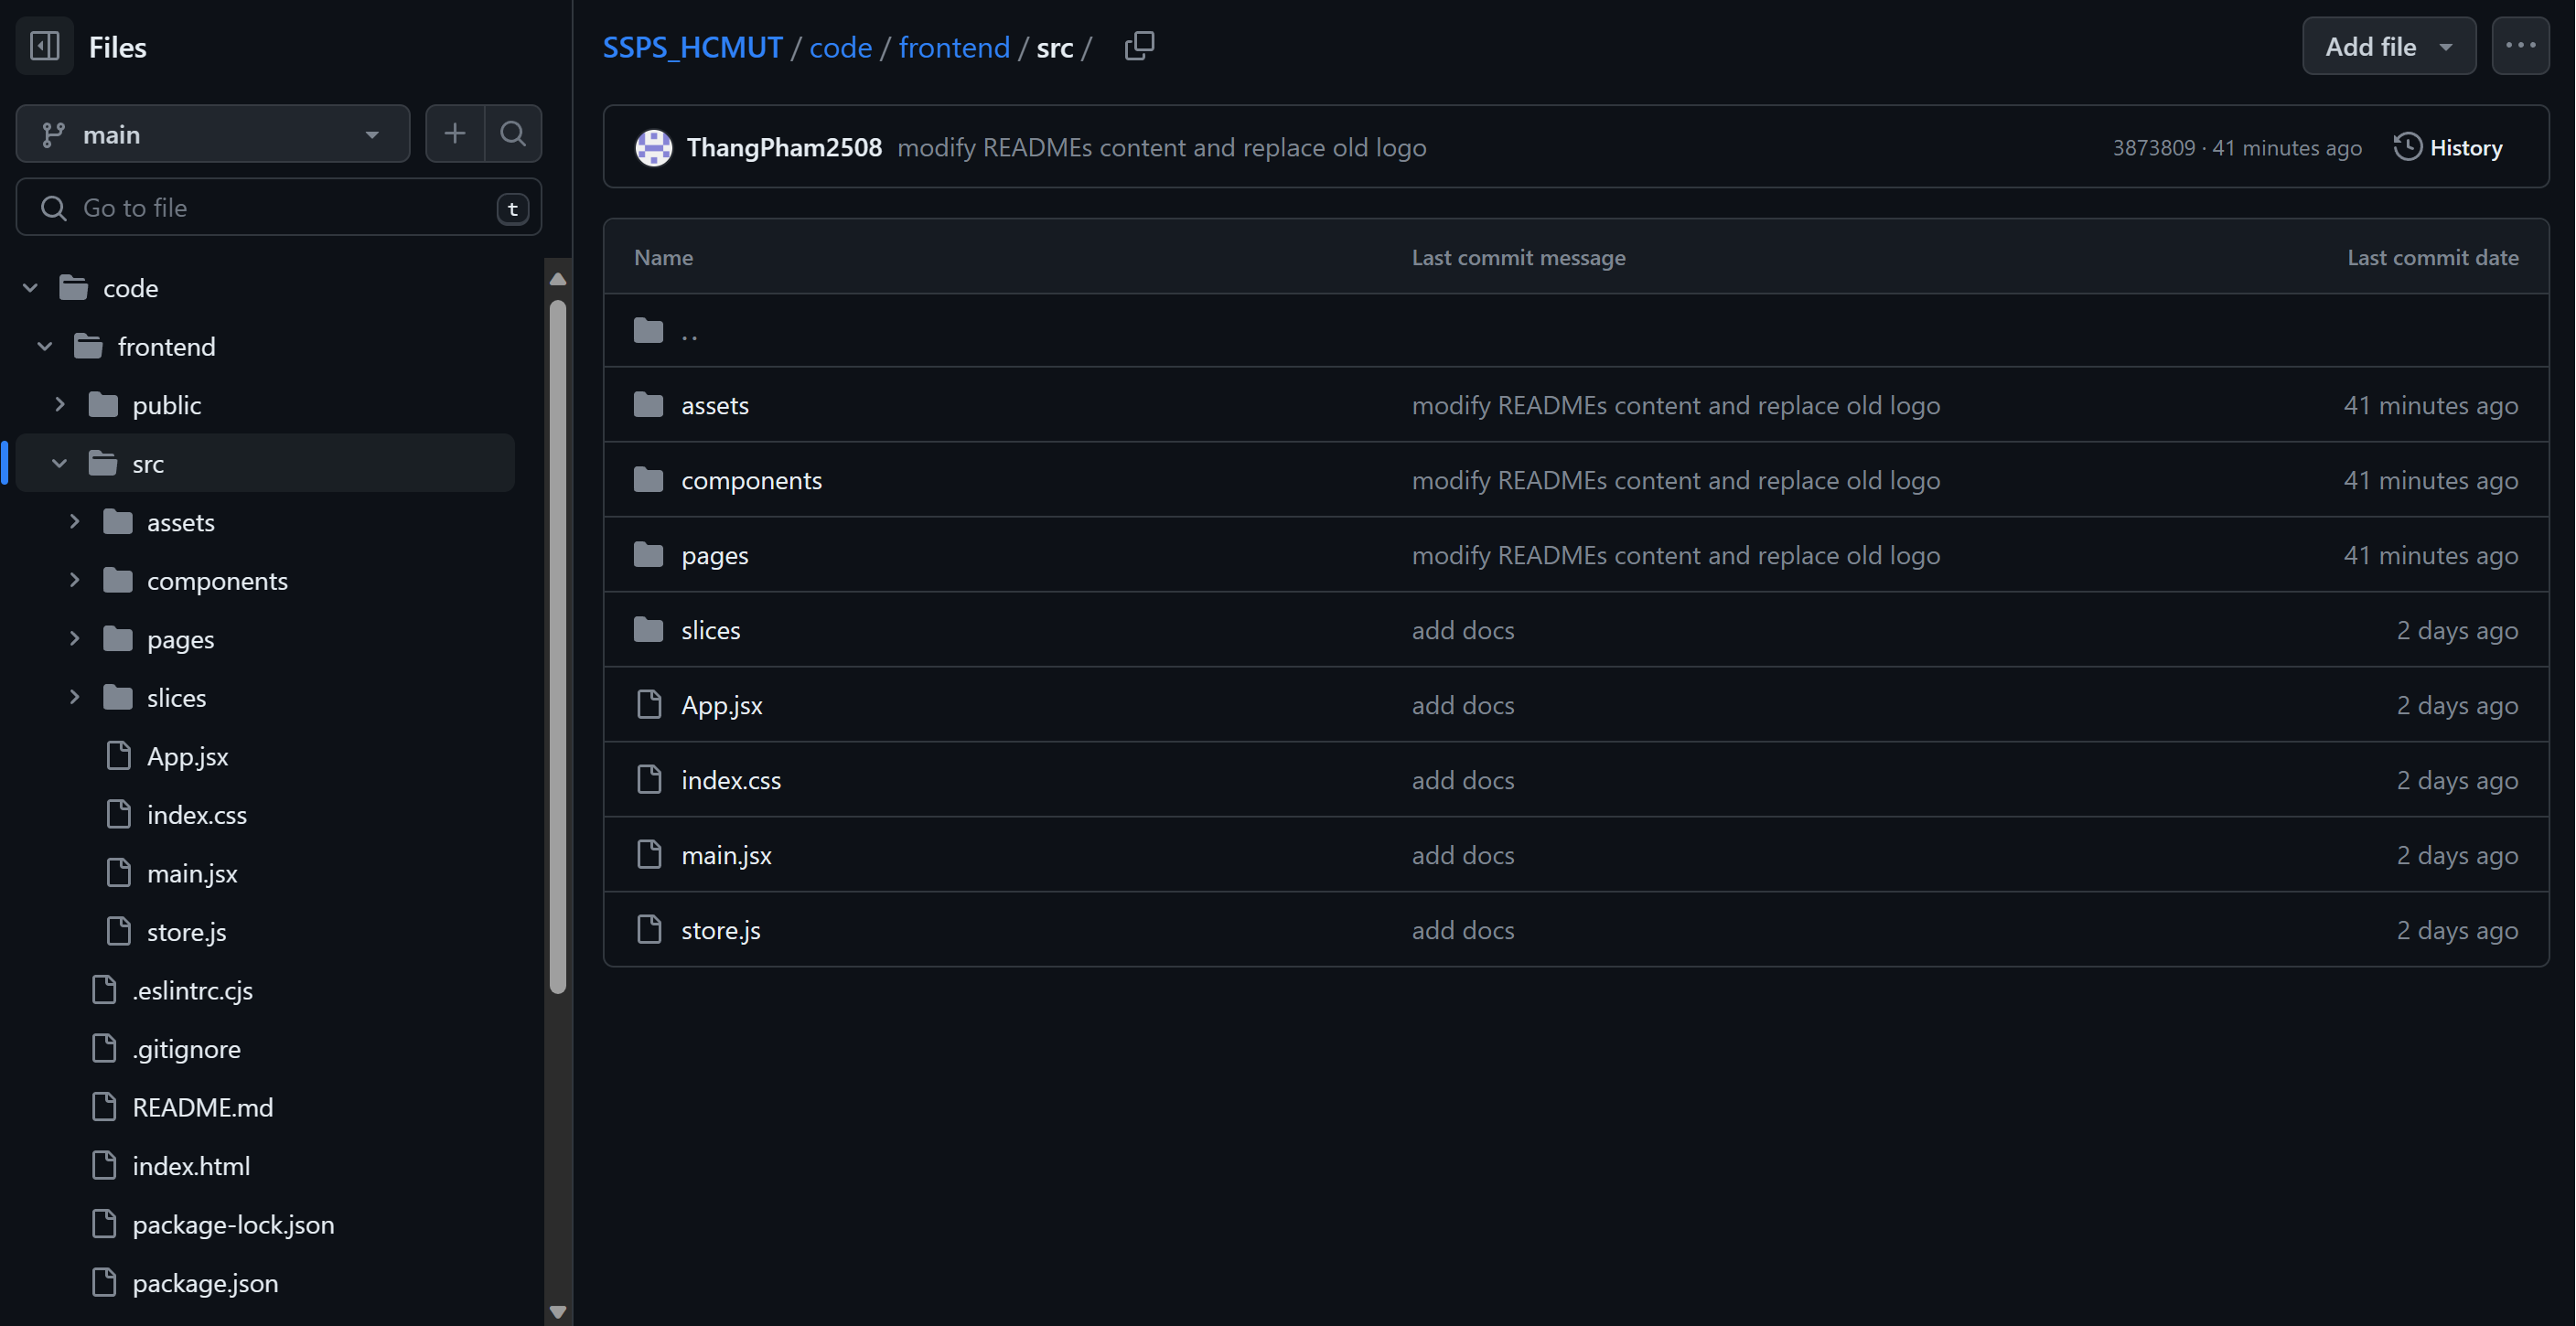
\includegraphics[width=1\textwidth]{Images/Github/github-src.png}
            \caption{Thư mục src}
        \end{center}
    \end{figure}
    \item \textbf{backend:} Thư mục này sẽ chứa mã nguồn cho máy chủ back-end, đó sẽ xử lý việc giao tiếp với máy in và cơ sở dữ liệu (sẽ được thêm sau).
    \end{itemize}
\end{itemize}

\subsection{Usability test bằng MVP1. Tổng hợp phản hồi và cải thiện}
\subsubsection{Tiến hành kiển tra việc sử dụng với UI được phát triển trong MVP1}
Để tiến hành kiểm tra, nhóm tác giả quyết định tạo một nền tảng và lấy khảo sát từ mọi người về sử dụng website của nhóm đế thấy được liệu họ có thích nó không. Thì nhóm nhận thấy hầu hết người dùng cảm thấy thoải mái với giao diện người dùng của MVP1 và chỉ cần cải tiến một chút là có thể có cái nhìn tốt hơn ở MVP2. Figma thì khá là khó để chứng minh cho người dùng thấy rằng ta tính làm gì với website. Các câu hỏi trên biểu mẫu google được dùng chủ yếu để lấy ý kiến sơ bộ hoặc cơ bản về giao diện người dùng theo quan điểm của họ. Sau cuộc khảo sát, nhóm tác giả đã thực hiện những thay đổi để làm cho hệ thống thân thiện hơn với người sử dụng và phục vụ trải nghiệm người dùng tốt hơn.\par
Biểu mẫu: 
\href{https://docs.google.com/forms/d/e/1FAIpQLSejZuRVfBreTUDDnRW45Cg20We1oYlPJiCv3Yp35g0XOEqzxw/viewform?fbclid=IwAR1cAii_2AATn-scg2h8SiijKK27mD7wnDgE8fzifFTZD-0UNnXU7ai2E8E}{Link khảo sát}.
\subsubsubsection{Trang chủ}
\begin{figure}[H]
    \begin{center}
        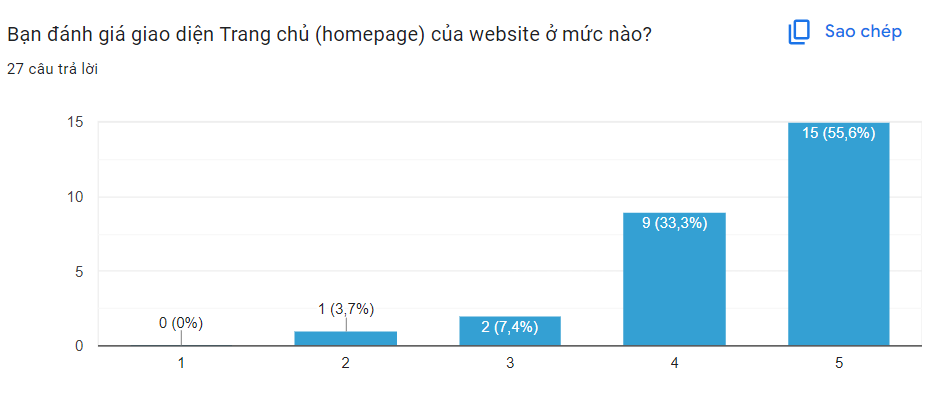
\includegraphics[width=1\textwidth]{Images/Test/test1.png}
        \caption{Khảo sát giao diện Trang chủ}
    \end{center}
\end{figure}
\subsubsubsection{Đăng nhập}
\begin{figure}[H]
    \begin{center}
        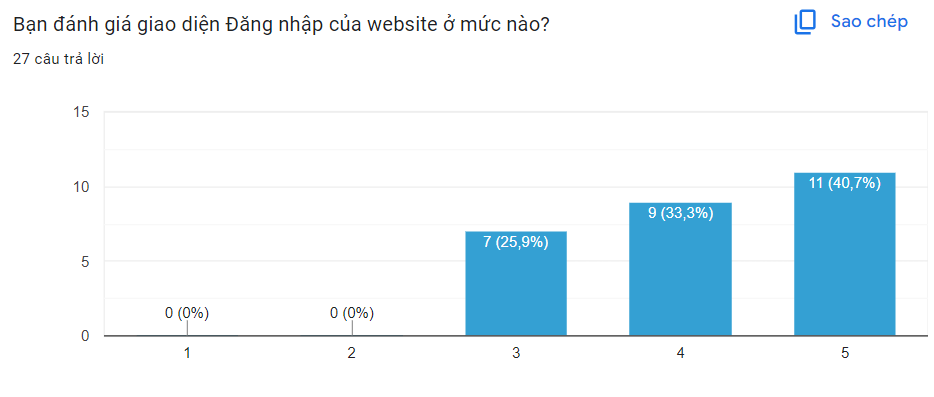
\includegraphics[width=1\textwidth]{Images/Test/test2.png}
        \caption{Khảo sát giao diện Đăng nhập}
    \end{center}
\end{figure}
\subsubsubsection{In ngay}
\begin{figure}[H]
    \begin{center}
        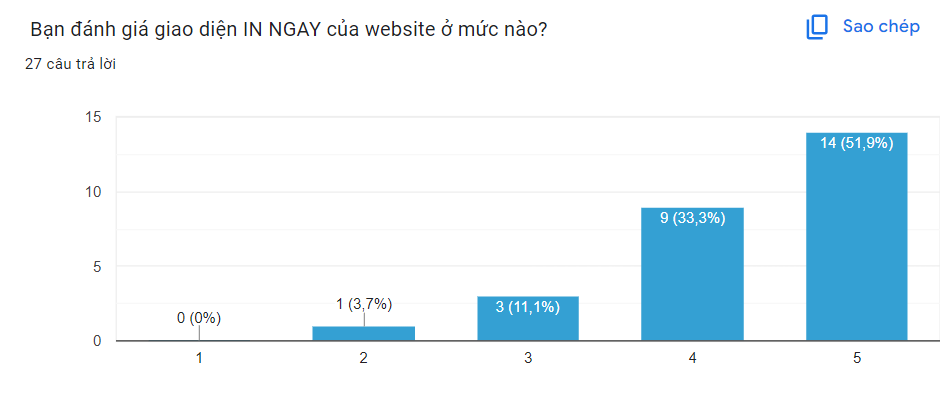
\includegraphics[width=1\textwidth]{Images/Test/test3.png}
        \caption{Khảo sát giao diện In ngay}
    \end{center}
\end{figure}
\subsubsubsection{Xem trước và cấu hình file in}
\begin{figure}[H]
    \begin{center}
        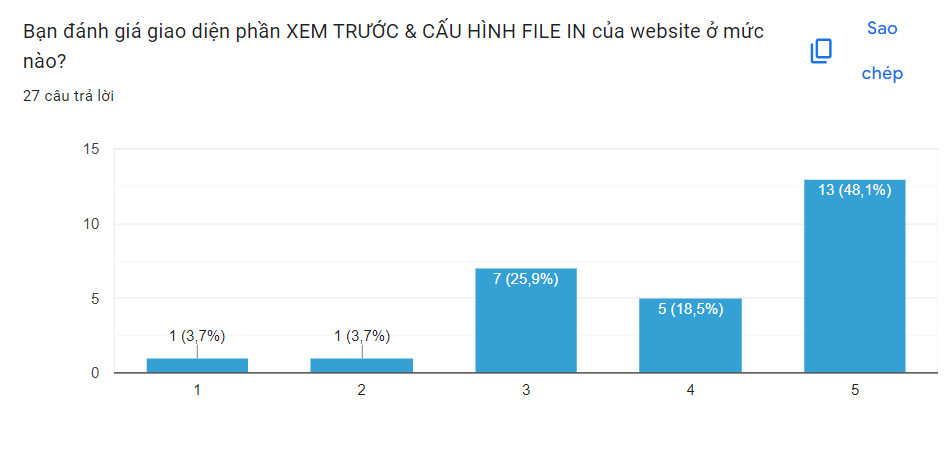
\includegraphics[width=1\textwidth]{Images/Test/test4.png}
        \caption{Khảo sát giao diện Xem trước và cấu hình file in}
    \end{center}
\end{figure}
\subsubsubsection{Quản lý máy in}
\begin{figure}[H]
    \begin{center}
        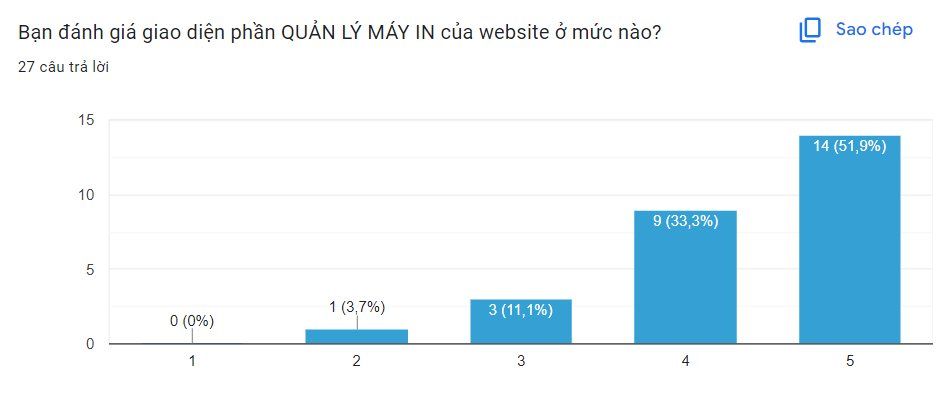
\includegraphics[width=1\textwidth]{Images/Test/test5.png}
        \caption{Khảo sát giao diện Quản lý máy in}
    \end{center}
\end{figure}
\subsubsubsection{Thêm máy in}
\begin{figure}[H]
    \begin{center}
        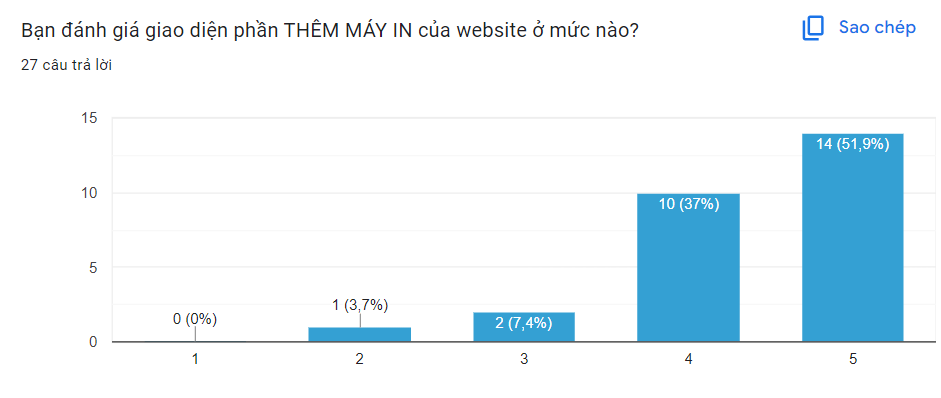
\includegraphics[width=1\textwidth]{Images/Test/test6.png}
        \caption{Khảo sát giao diện Thêm máy in}
    \end{center}
\end{figure}
\subsubsubsection{Lịch sử in ấn}
\begin{figure}[H]
    \begin{center}
        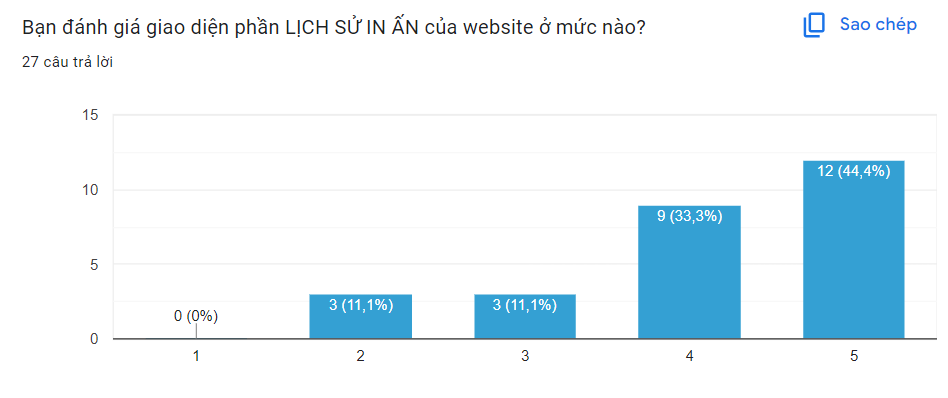
\includegraphics[width=1\textwidth]{Images/Test/test7.png}
        \caption{Khảo sát giao diện Lịch sử in ấn}
    \end{center}
\end{figure}
\subsubsubsection{Mua giấy in}
\begin{figure}[H]
    \begin{center}
        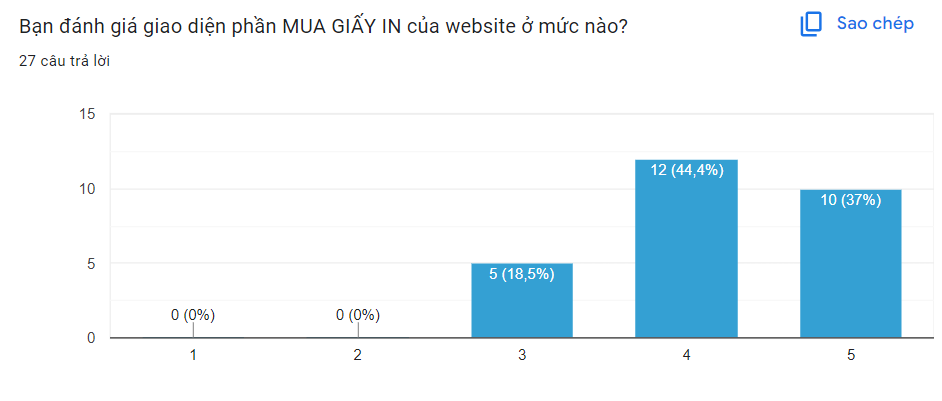
\includegraphics[width=1\textwidth]{Images/Test/test8.png}
        \caption{Khảo sát giao diện Mua giấy in}
    \end{center}
\end{figure}
\subsubsection{Tổng hợp phản hồi và cải thiện MVP1 thành MVP2 với trải nghiệm người dùng tốt hơn}
Nhìn chung thì phần trải nghiệm người dùng cho MVP1 khá ổn với điểm số được chấm từ 7 trở lên, điểm cao nhất là 10 chiếm ưu thế với 37\%, điểm 8 chiếm thứ 2 với 33.3\%.
\begin{figure}[H]
    \begin{center}
        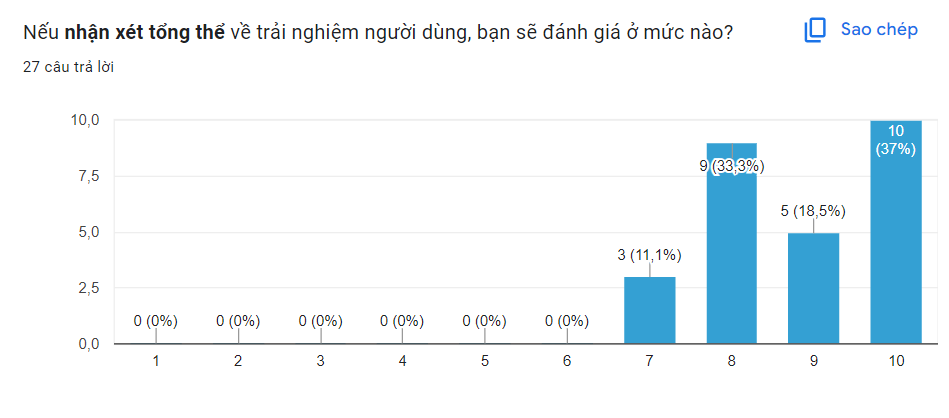
\includegraphics[width=1\textwidth]{Images/Test/test_total.png}
        \caption{Khảo sát về trải nghiệm người dùng cho MVP1}
    \end{center}
\end{figure}
Và nhóm cũng có khảo sát về việc sử dụng thành thạo website của một số người dùng thì nhận thấy phần lớn (70.4\%) là có thể sử dụng thành thạo mà không cần hướng dẫn chi tiết cụ thể. Tuy nhiên một số vẫn chưa thể với 25.9\% là không hẳn và 3.7\% chắc chắn không.
\begin{figure}[H]
    \begin{center}
        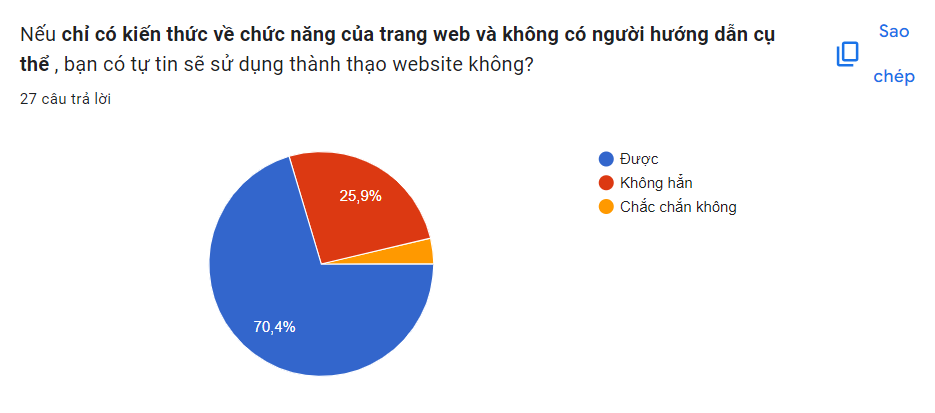
\includegraphics[width=1\textwidth]{Images/Test/test_tutoral.png}
        \caption{Khảo sát khả năng sử dụng thành thạo website không cần hướng dẫn}
    \end{center}
\end{figure}
Sau khi tóm tắt tất cả các phản hồi, chúng tôi đã đưa ra một số cải thiện về giao diện người dùng của mình:
\begin{itemize}
    \item Trang chủ: Sửa lại background của trang chủ cho dễ nhìn.
    \begin{figure}[H]
        \begin{center}
            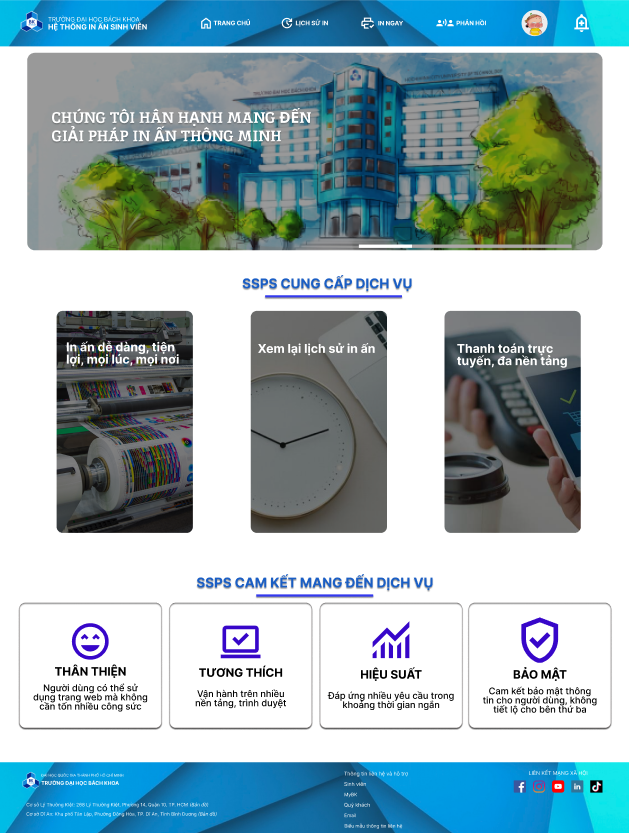
\includegraphics[width=0.7\textwidth]{Images/Test/fix_homepage.png}
            \caption{Cải thiện giao diện Trang chủ}
        \end{center}
    \end{figure}
    \item Button: Thống nhất lại màu sắc các nút bấm cho hài hòa, hút mắt người xem.
    \begin{figure}[H]
        \begin{center}
            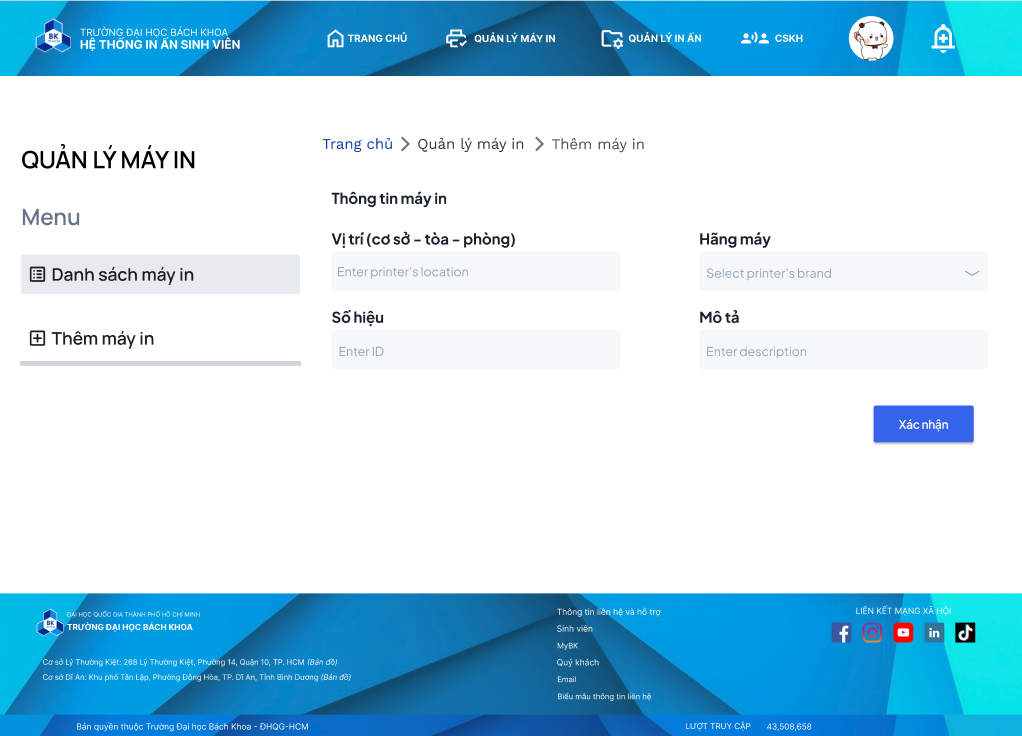
\includegraphics[width=1\textwidth]{Images/Test/fix_button.png}
            \caption{Cải thiện màu sắc các nút}
        \end{center}
    \end{figure}
    \item Lịch sử in ấn: Chỉnh sửa màu sắc cho đỡ chói và hài hòa hơn, sắp xếp mọi thứ có cấu trúc, đều đặn hơn.
    \begin{figure}[H]
        \begin{center}
            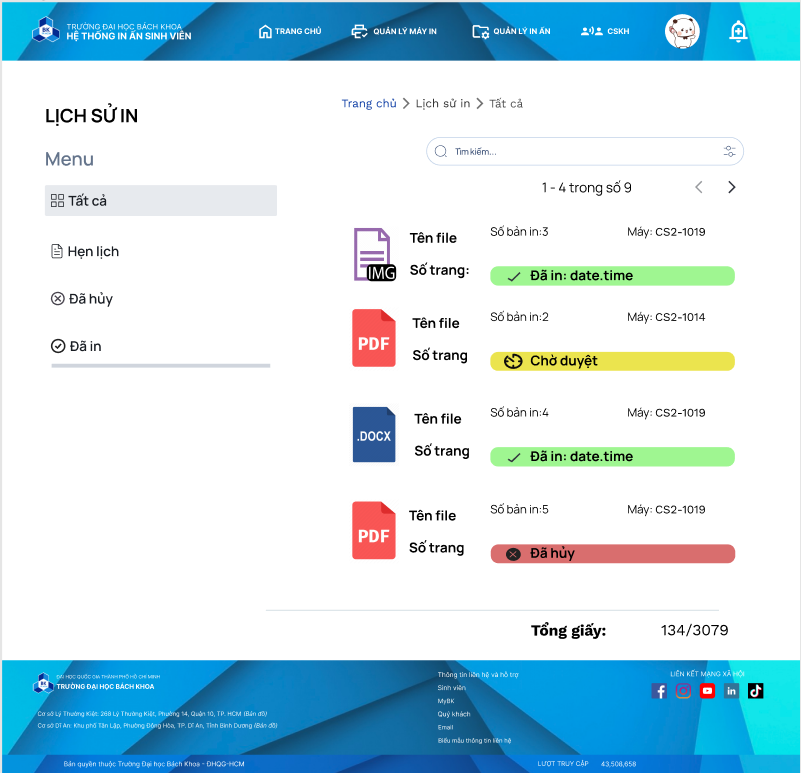
\includegraphics[width=1\textwidth]{Images/Test/fix_history.png}
            \caption{Cải thiện giao diện Lịch sử in ấn}
        \end{center}
    \end{figure}
    \item Mua giấy in: Chỉnh sửa cỡ chữ cho phù hợp hơn.
    \begin{figure}[H]
        \begin{center}
            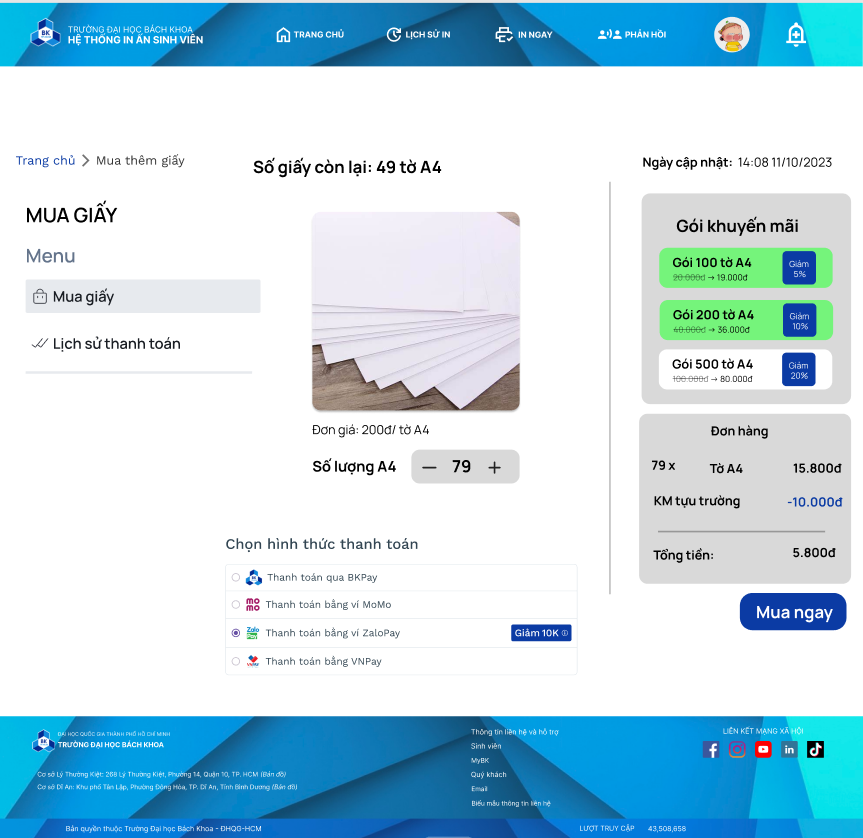
\includegraphics[width=1\textwidth]{Images/Test/fix_buypaper.png}
            \caption{Cải thiện giao diện Mua giấy in}
        \end{center}
    \end{figure}
\end{itemize}
